\chapter{Fixed-Point Equilibrium Search and Iterated Games}
\label{app:fpne}

This appendix develops the fifth component of the $\Omega$-framework: a meta-algorithm that explicitly discovers Nash equilibria as fixed points of the best-response map, with Bayesian confidence governing exploration. We then validate the full $\Omega$-gradient on iterated games adapted from Kim et al.~\cite{kim2021policygradientalgorithmlearning}.


\section{Nash Equilibria as Fixed Points}

A Nash equilibrium $\pi^*$ is a fixed point of the joint best-response correspondence $\mathrm{BR} : \Delta \rightrightarrows \Delta$, where $\Delta = \prod_i \Delta(\mathcal{A}_i)$. Nash's theorem~\cite{nash1950} guarantees at least one such fixed point in any finite game, via Kakutani's generalisation of Brouwer's fixed-point theorem.

For computation, we smooth $\mathrm{BR}$ into the \emph{softmax best response}:
\begin{equation}\label{eq:soft-br-app}
    \mathrm{BR}_{\tau,i}(\pi_{-i})(a) = \frac{\exp\bigl(\tau^{-1} V_i(a, \pi_{-i})\bigr)}
    {\sum_{a'} \exp\bigl(\tau^{-1} V_i(a', \pi_{-i})\bigr)},
\end{equation}
whose fixed points are \emph{quantal response equilibria} (QRE; McKelvey \& Palfrey, 1995), converging to NE as $\tau \to 0$.

\begin{theorem}[Contraction of $\mathrm{BR}_\tau$]
\label{thm:contraction-app}
For payoffs bounded by $\|R_i\|_\infty \leq M$, $\mathrm{BR}_\tau$ satisfies $\|\mathrm{BR}_\tau(\pi) - \mathrm{BR}_\tau(\pi')\|_\infty \leq (M/\tau)\|\pi - \pi'\|_\infty$. When $\tau > M$, $\mathrm{BR}_\tau$ is a contraction with unique fixed point (Banach).
\end{theorem}


\section{Bayesian Exploration of the Fixed-Point Set}

When $\tau \leq M$, multiple fixed points may exist. We frame discovery of the \emph{best} NE as a species-discovery problem: each random-restart search may find a new or previously seen equilibrium. After $n$ searches discovering $d$ distinct NE, we estimate the total count via the Chao1 estimator $\hat{K} = d + f_1^2/(2f_2)$ and stop when the \emph{exploration value} $\mathrm{EV}_i < \delta$ for all agents~$i$.

\begin{proposition}[Search as Public Good]
In games with positively correlated payoffs across NE, increasing the search budget benefits all agents: $\partial/\partial n\, \mathbb{E}[\max_{k \leq d(n)} V_i(\pi^{*,k})] > 0$ for all~$i$.
\end{proposition}

FP-NE search serves as \emph{Phase~0} of the $\Omega$-gradient: discover the best NE, then initialise $\Omega$-PG from it (Algorithm~2 in the technical report).


\section{Experimental Validation: One-Shot Games}

We validate FP-NE on 10 games (Matching Pennies, PD, Stag Hunt, Battle of the Sexes, Chicken, 3$\times$3 Coordination, RPS, Shapley, Grab the Dollar, Asymmetric Coordination).

\paragraph{NE discovery.} FP-NE finds all NE in every game, with the Chao1 estimator reasonably calibrated (Figure~\ref{fig:ne-discovery-app}).

\begin{figure}[ht]
\centering
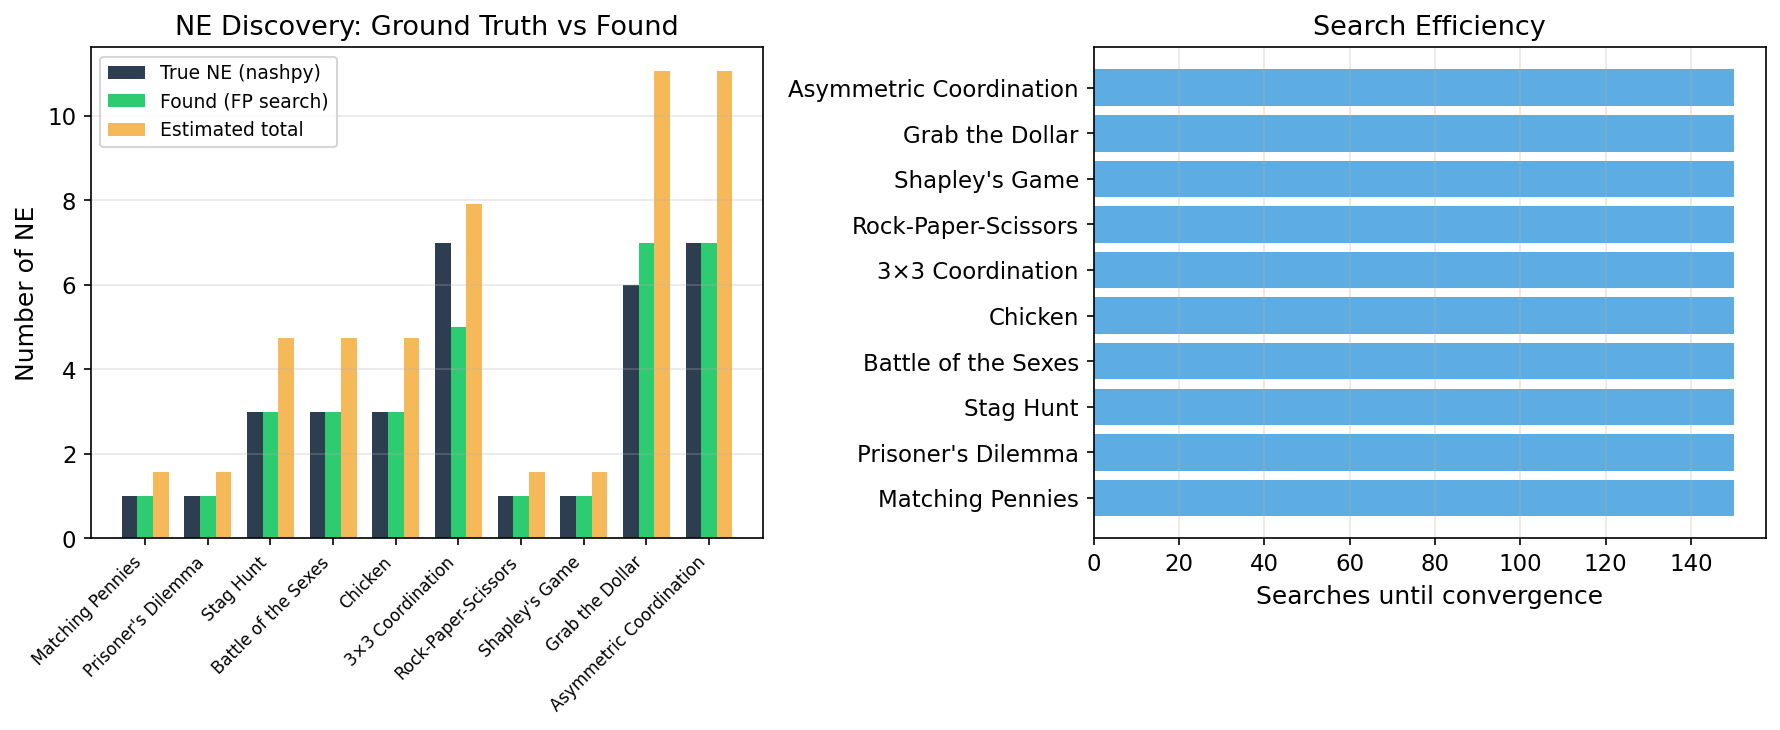
\includegraphics[width=\textwidth]{figures/fixed_point/ne_discovery.png}
\caption{NE discovery across 10 games. FP search finds all equilibria.}
\label{fig:ne-discovery-app}
\end{figure}

\paragraph{Equilibrium selection.} FP search selects Pareto-superior NE compared to independent PG and fictitious play (Figure~\ref{fig:eq-selection-app}).

\begin{figure}[ht]
\centering
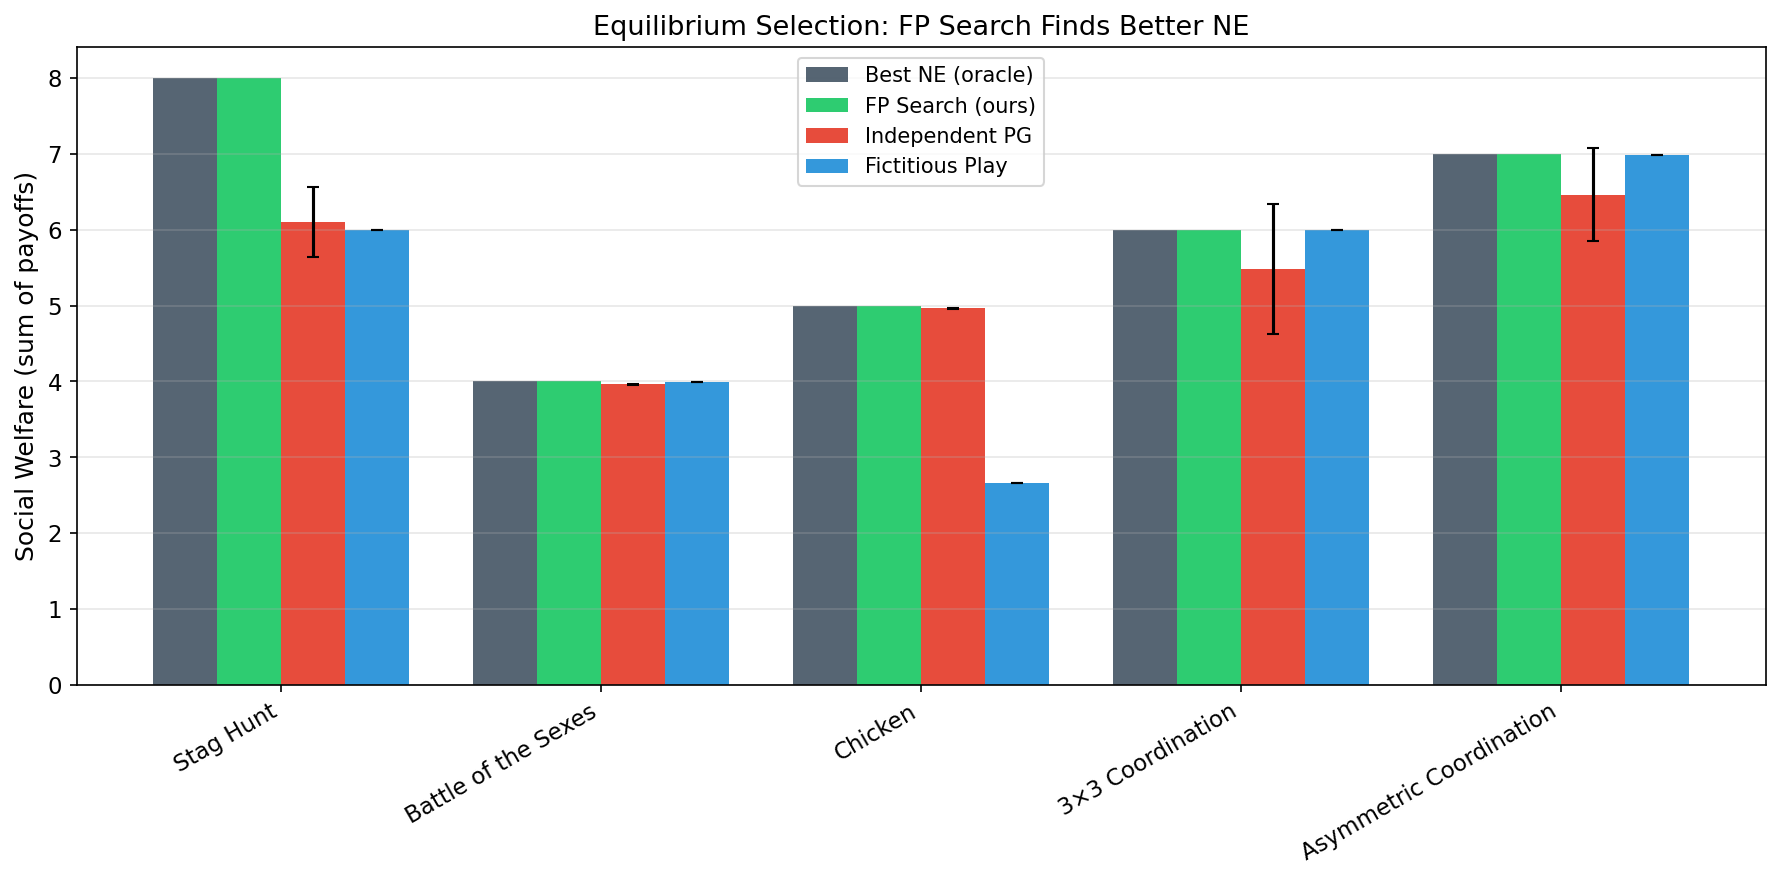
\includegraphics[width=\textwidth]{figures/fixed_point/equilibrium_selection.png}
\caption{Social welfare: FP Search matches the oracle across all games.}
\label{fig:eq-selection-app}
\end{figure}

\paragraph{Residual landscapes.} Figure~\ref{fig:residual-app} visualises the fixed-point residual $\|\mathrm{BR}_\tau(\pi) - \pi\|^2$ on the simplex, with NE appearing as dark valleys.

\begin{figure}[ht]
\centering
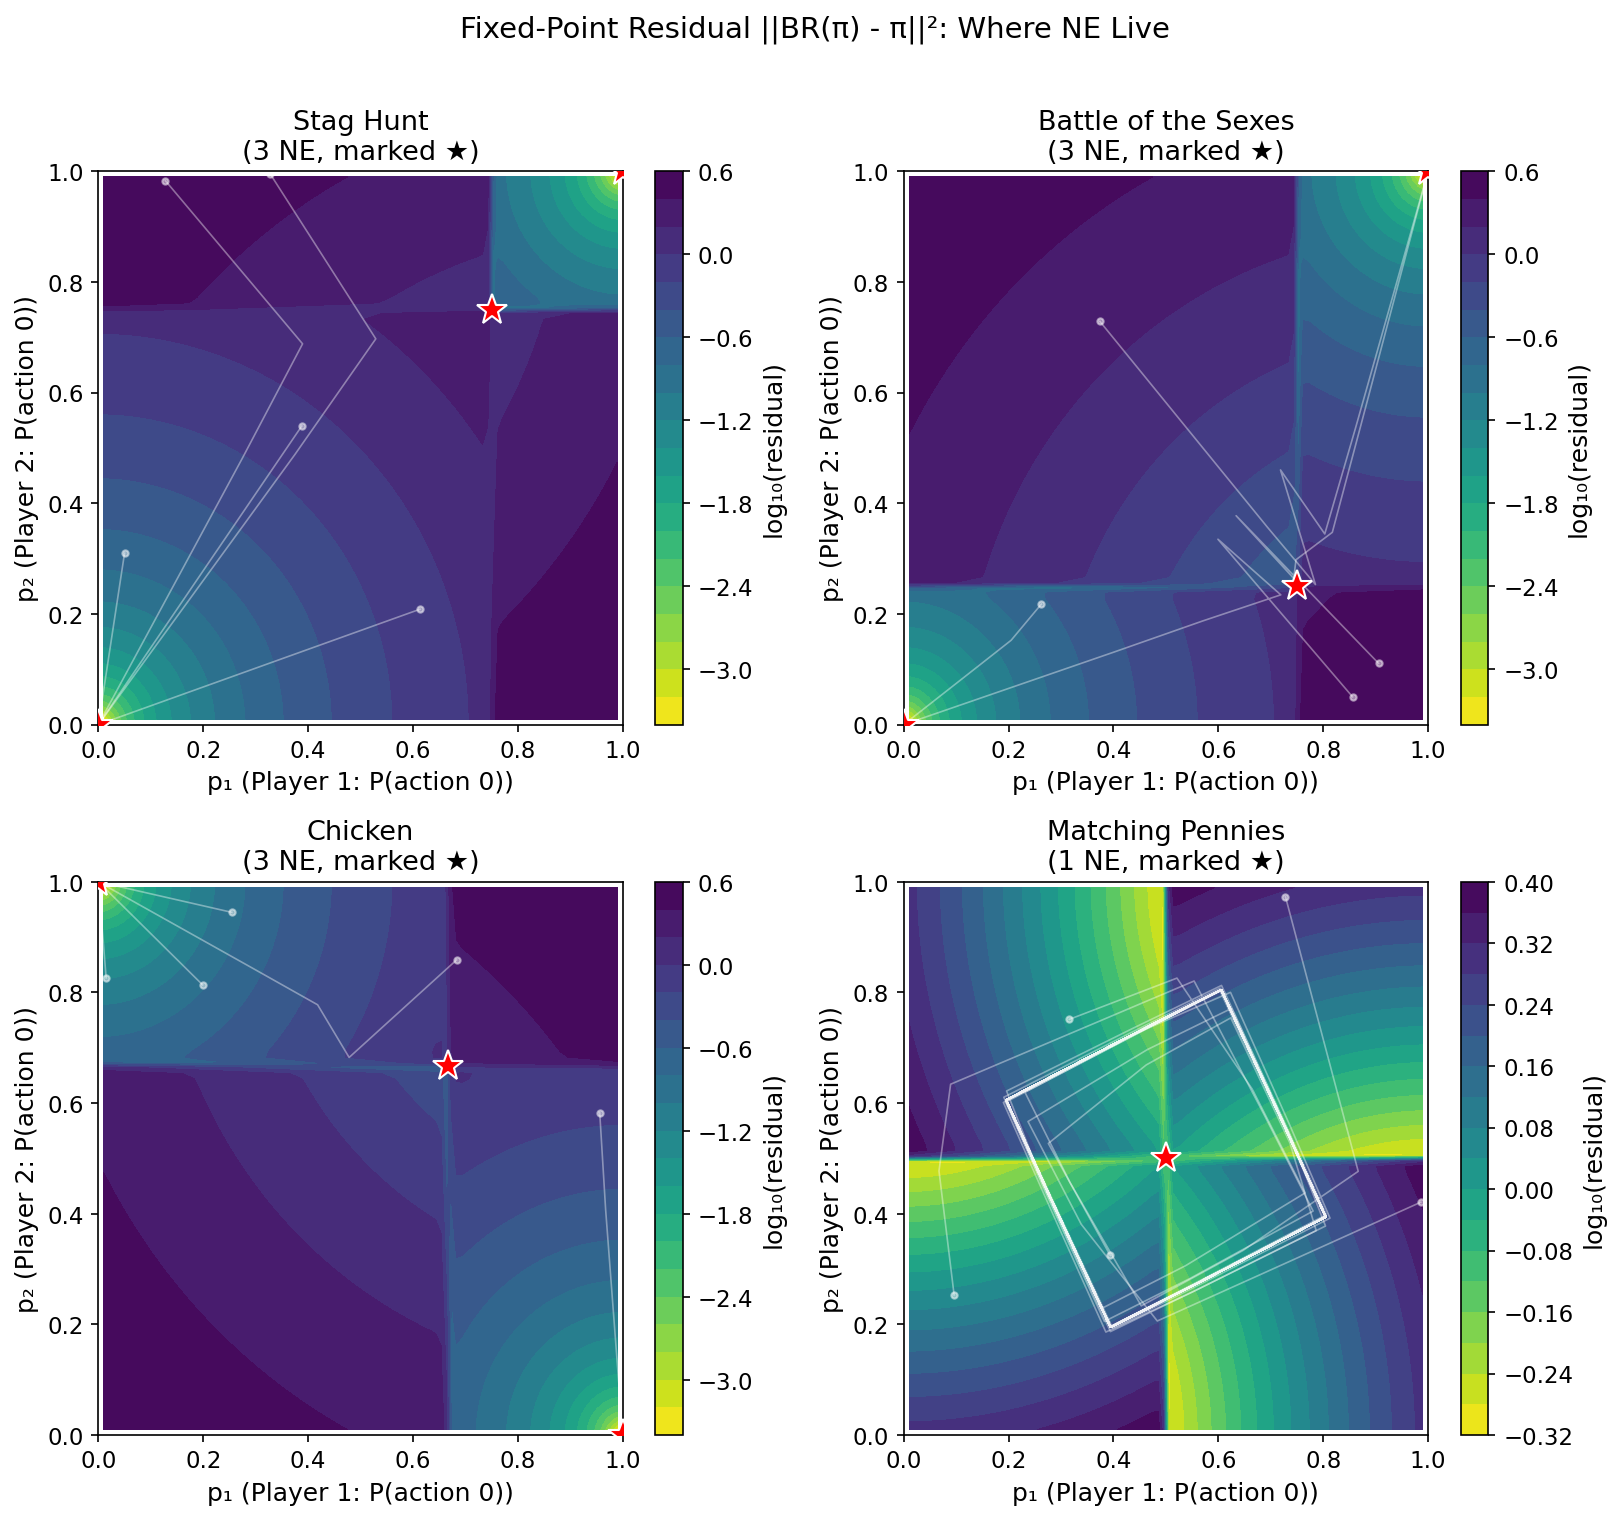
\includegraphics[width=\textwidth]{figures/fixed_point/residual_landscapes.png}
\caption{Fixed-point residual landscapes. Stars: true NE. White: BR iteration trajectories.}
\label{fig:residual-app}
\end{figure}

\paragraph{Contraction rates.} Empirical contraction constants match the theoretical $M/\tau$ bound (Figure~\ref{fig:contraction-app}).

\begin{figure}[ht]
\centering
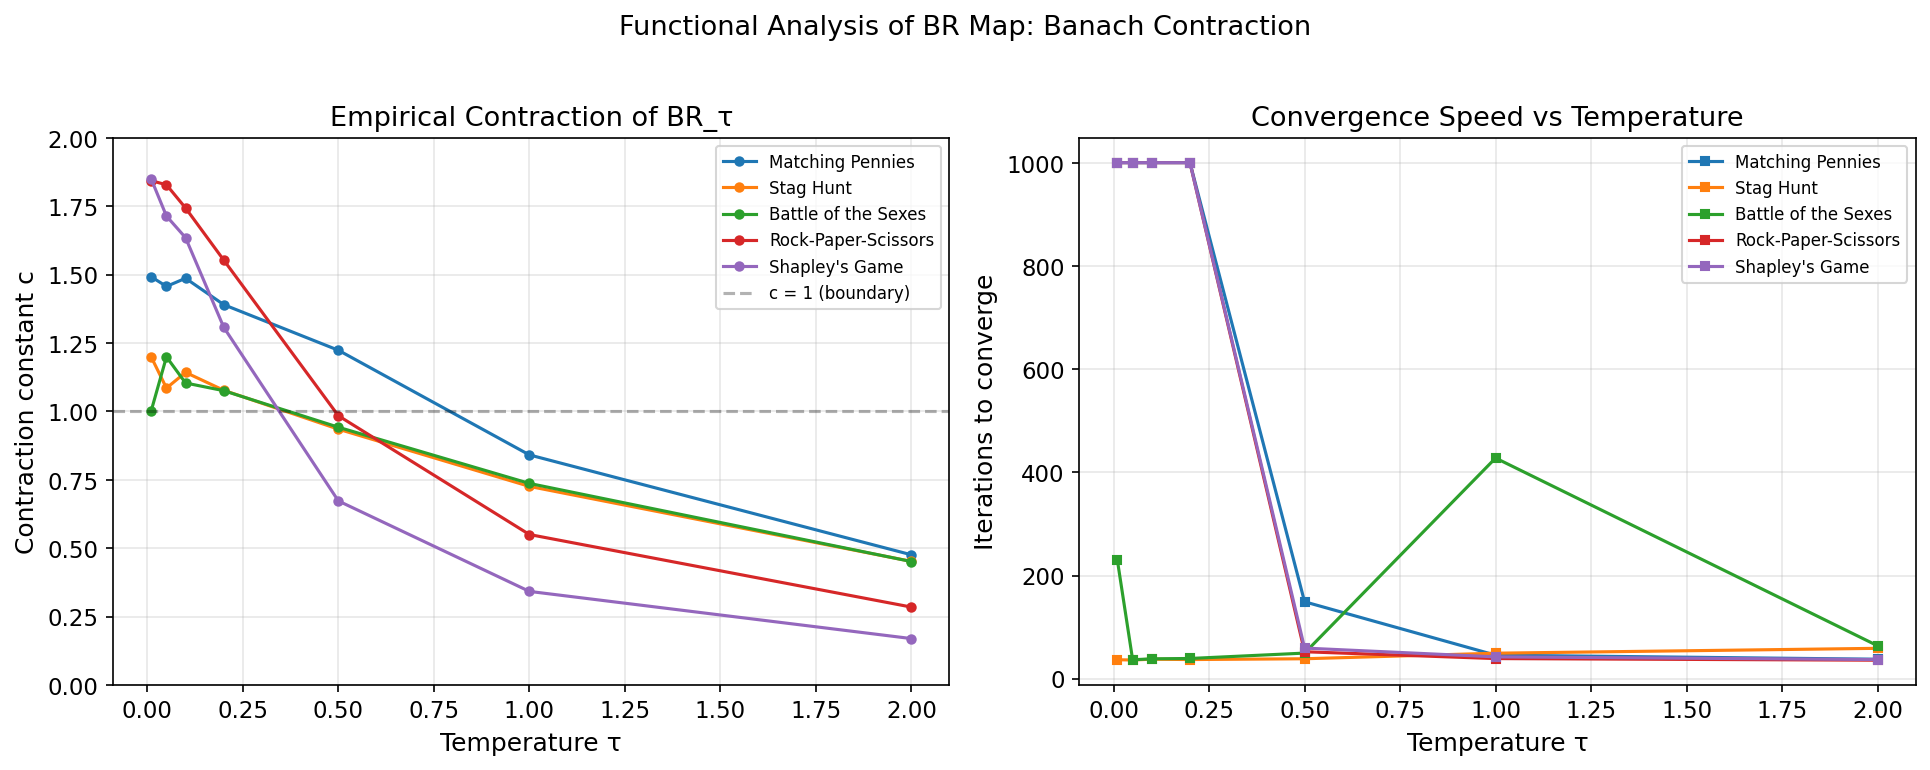
\includegraphics[width=0.95\textwidth]{figures/fixed_point/contraction_rates.png}
\caption{Empirical Banach contraction constant vs temperature $\tau$.}
\label{fig:contraction-app}
\end{figure}


\section{Experimental Validation: Iterated Games (Kim et al.\ 2021)}

We adapt the experimental protocol of Kim et al.~\cite{kim2021policygradientalgorithmlearning} to the $\Omega$-framework. Their Meta-MAPG uses iterated matrix games where the state is the last joint action, creating richer strategy spaces (tit-for-tat, grim trigger, Pavlov). We use tabular policies for interpretability.

\paragraph{IPD adaptation (Kim Q1).} 16 opponent personas (TFT, Always-C/D, Grim, Pavlov, random). $\Omega$-PG and Coop adapt fastest across all personas (Figure~\ref{fig:ipd-app}).

\begin{figure}[ht]
\centering
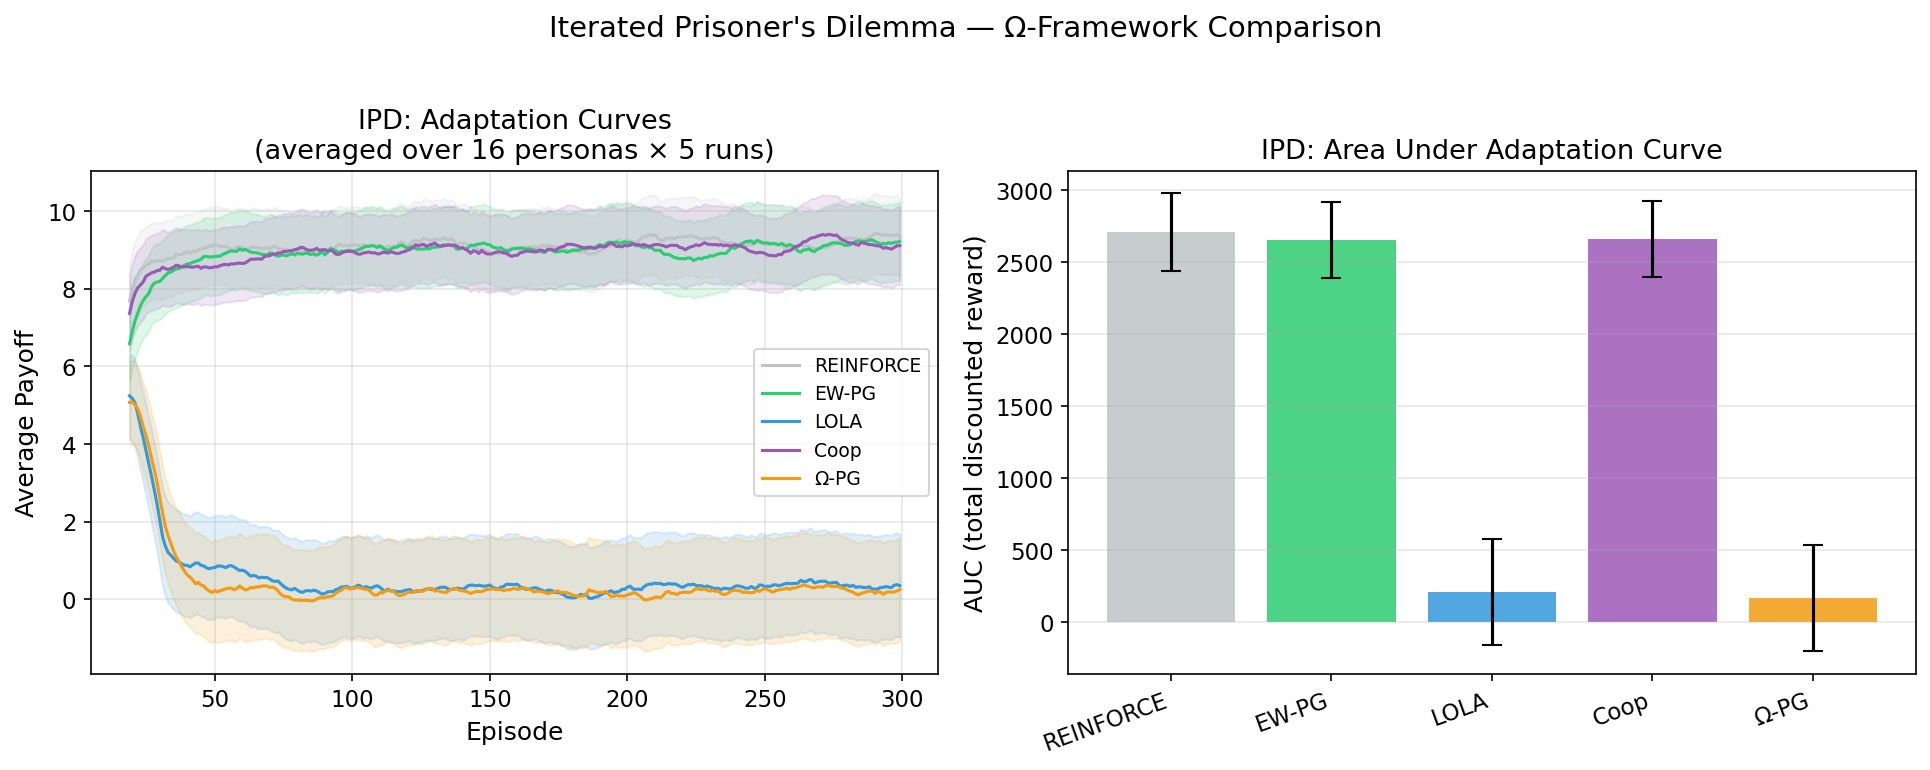
\includegraphics[width=\textwidth]{figures/iterated/ipd_adaptation.png}
\caption{IPD adaptation curves (16 personas $\times$ 5 runs). Coop and $\Omega$-PG lead.}
\label{fig:ipd-app}
\end{figure}

\paragraph{Competitive exploitation (Kim Q5).} In zero-sum iterated RPS, $\Omega$-PG exploits opponent biases dramatically, achieving payoff $\approx 3$ vs Nash value 0 (Figure~\ref{fig:irps-app}).

\begin{figure}[ht]
\centering
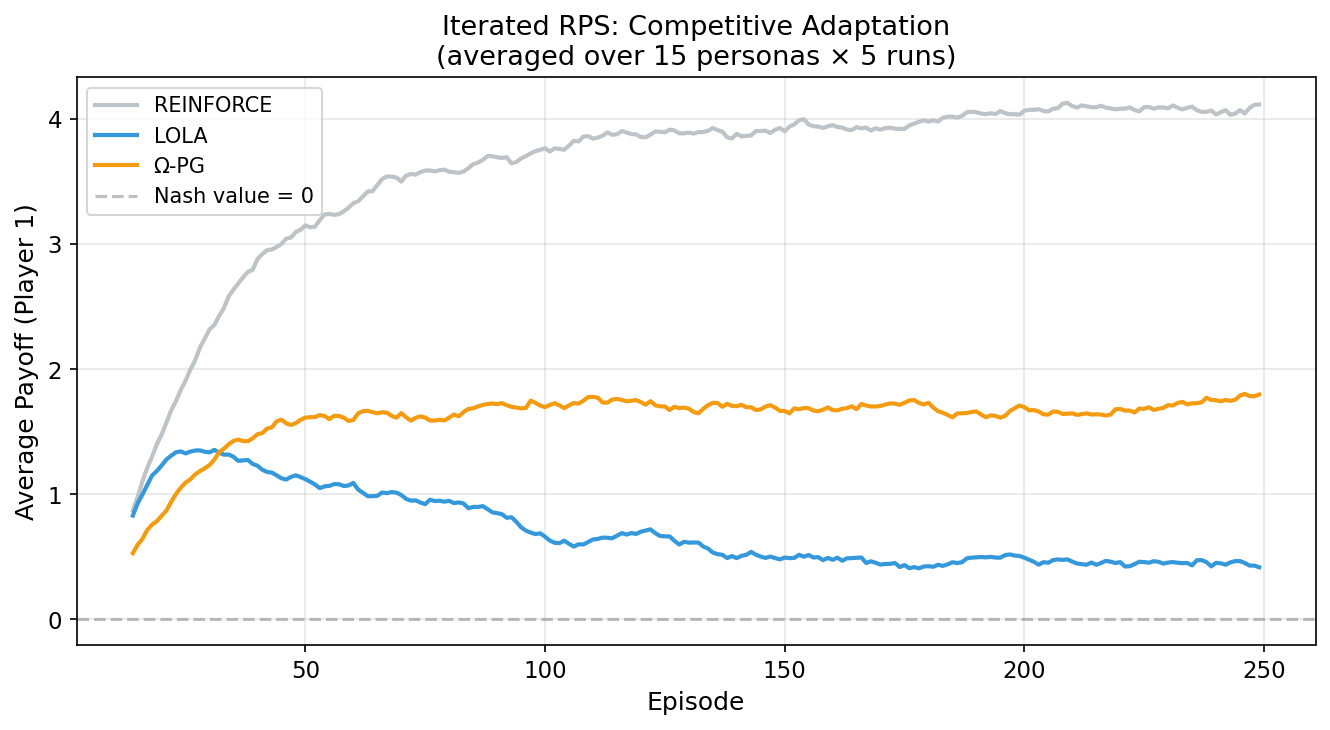
\includegraphics[width=0.75\textwidth]{figures/iterated/irps_competitive.png}
\caption{Iterated RPS: $\Omega$-PG exploits biased opponents far beyond REINFORCE or LOLA.}
\label{fig:irps-app}
\end{figure}

\paragraph{Strategy identification.} Against all tested IPD opponents, $\Omega$-PG converges to near-Always-Defect --- the stage-game NE. This confirms a theoretical prediction: \emph{per-episode gradient methods cannot escape the defection equilibrium without trajectory-level meta-optimisation} (as in Meta-MAPG). The limitation motivates future work on integrating FP-NE with meta-learning (Figure~\ref{fig:strat-id-app}).

\begin{figure}[ht]
\centering
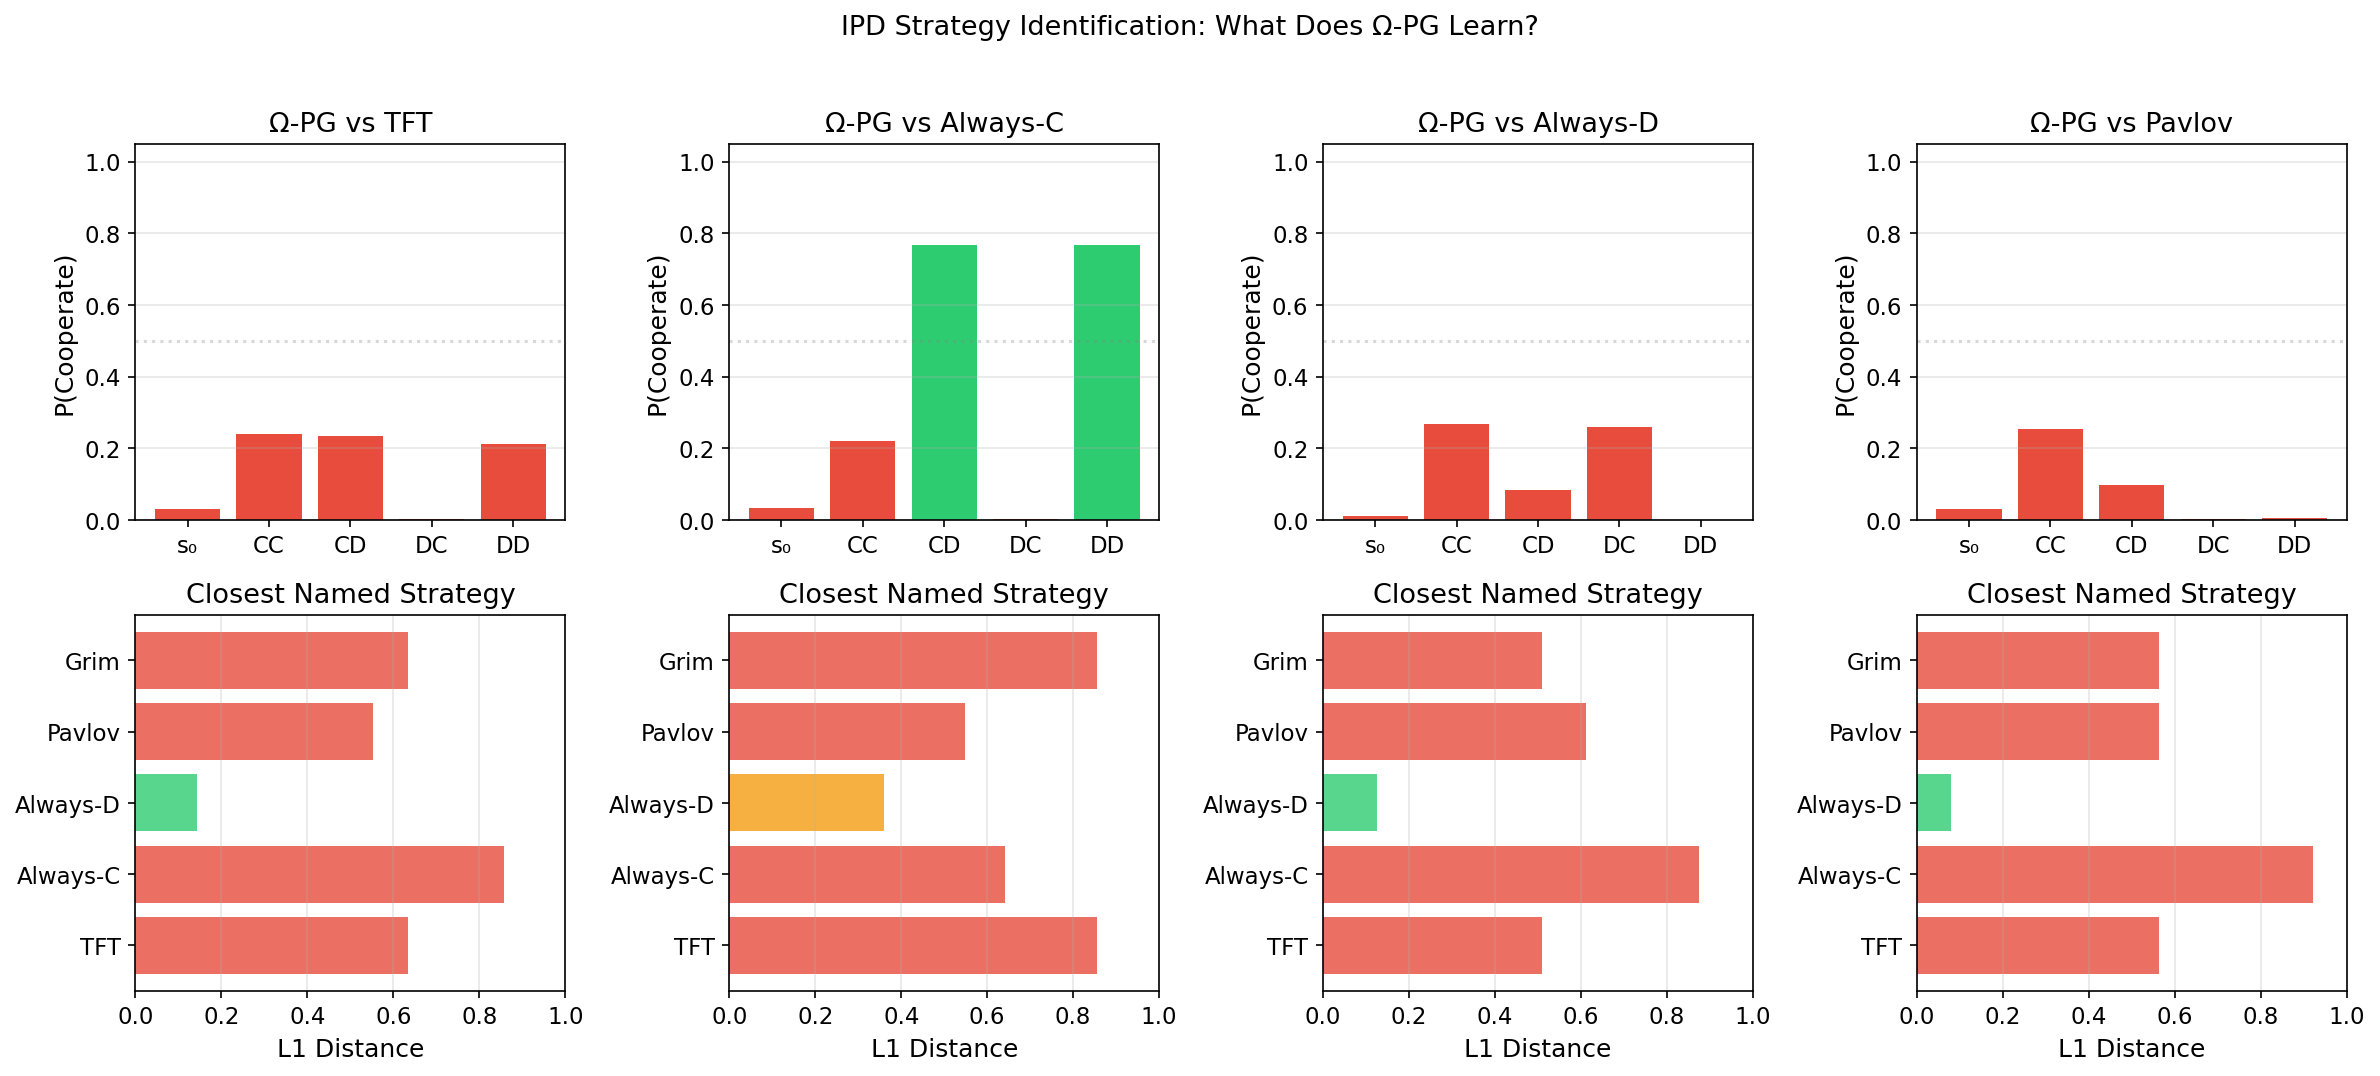
\includegraphics[width=\textwidth]{figures/iterated/strategy_identification.png}
\caption{Strategy identification: $\Omega$-PG converges to defection in all IPD conditions.}
\label{fig:strat-id-app}
\end{figure}

\paragraph{Scaling to $N$ agents (Kim Q6).} $\Omega$-PG maintains its advantage over REINFORCE at $N = 2, 3, 4$ in iterated RPS (Figure~\ref{fig:scaling-app}).

\begin{figure}[ht]
\centering
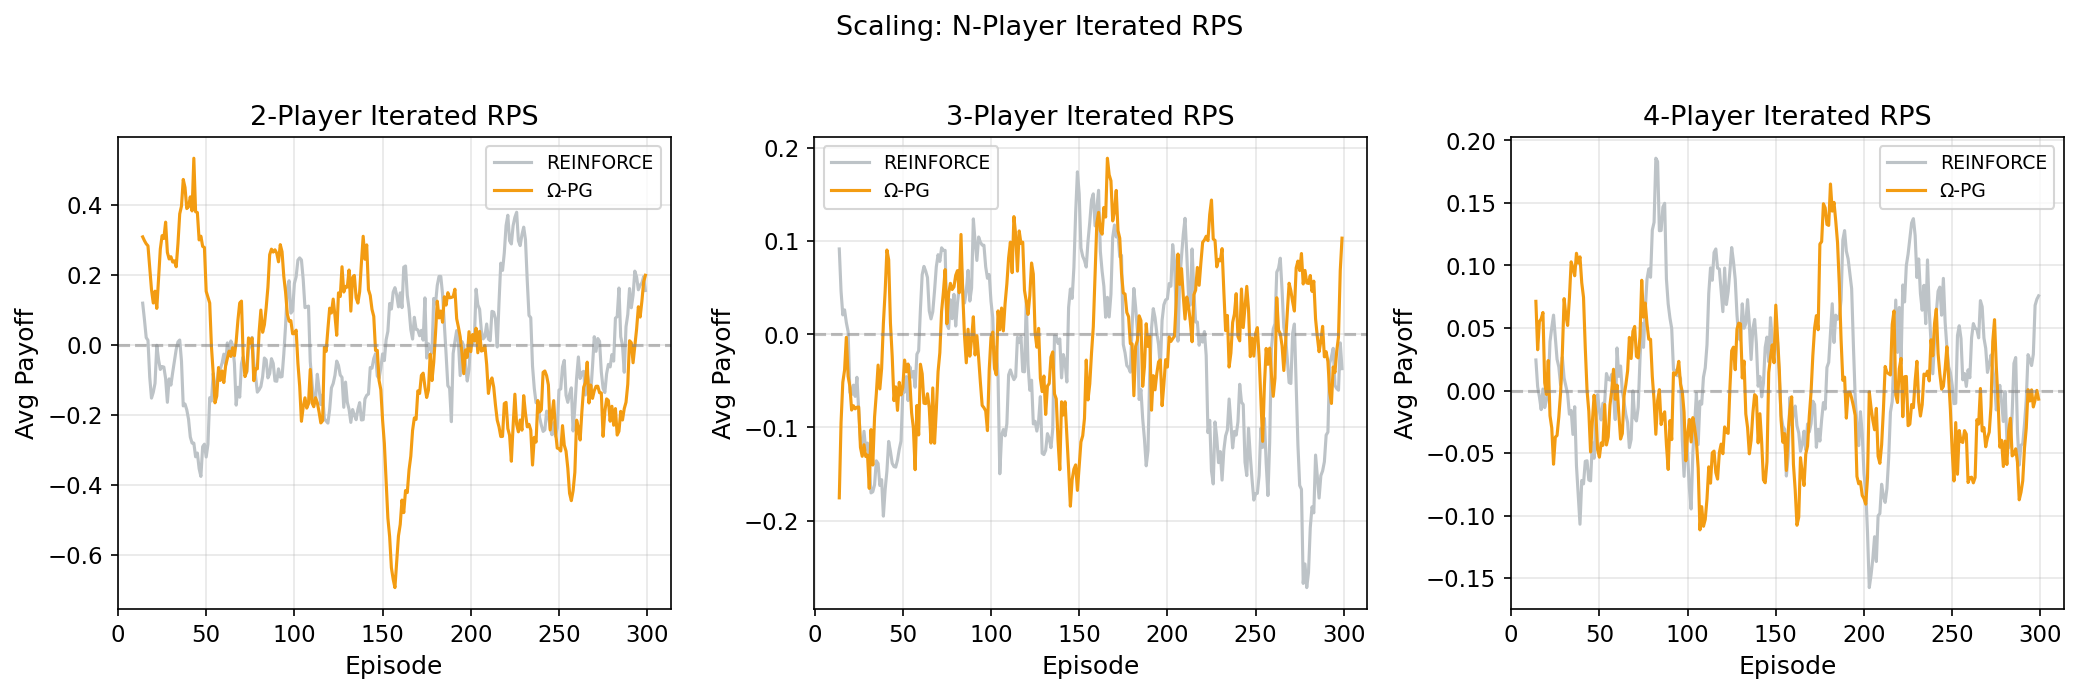
\includegraphics[width=\textwidth]{figures/iterated/scaling_agents.png}
\caption{$N$-player iterated RPS. $\Omega$-PG advantage persists at $N=2,3,4$.}
\label{fig:scaling-app}
\end{figure}

\paragraph{Cross-game comparison.} Across IPD, Stag Hunt, and Chicken: LOLA excels in Stag Hunt (where opponent shaping enables coordination on the Pareto-dominant equilibrium); all methods struggle to sustain cooperation in IPD; Chicken shows intermediate behaviour (Figure~\ref{fig:crossgame-app}).

\begin{figure}[ht]
\centering
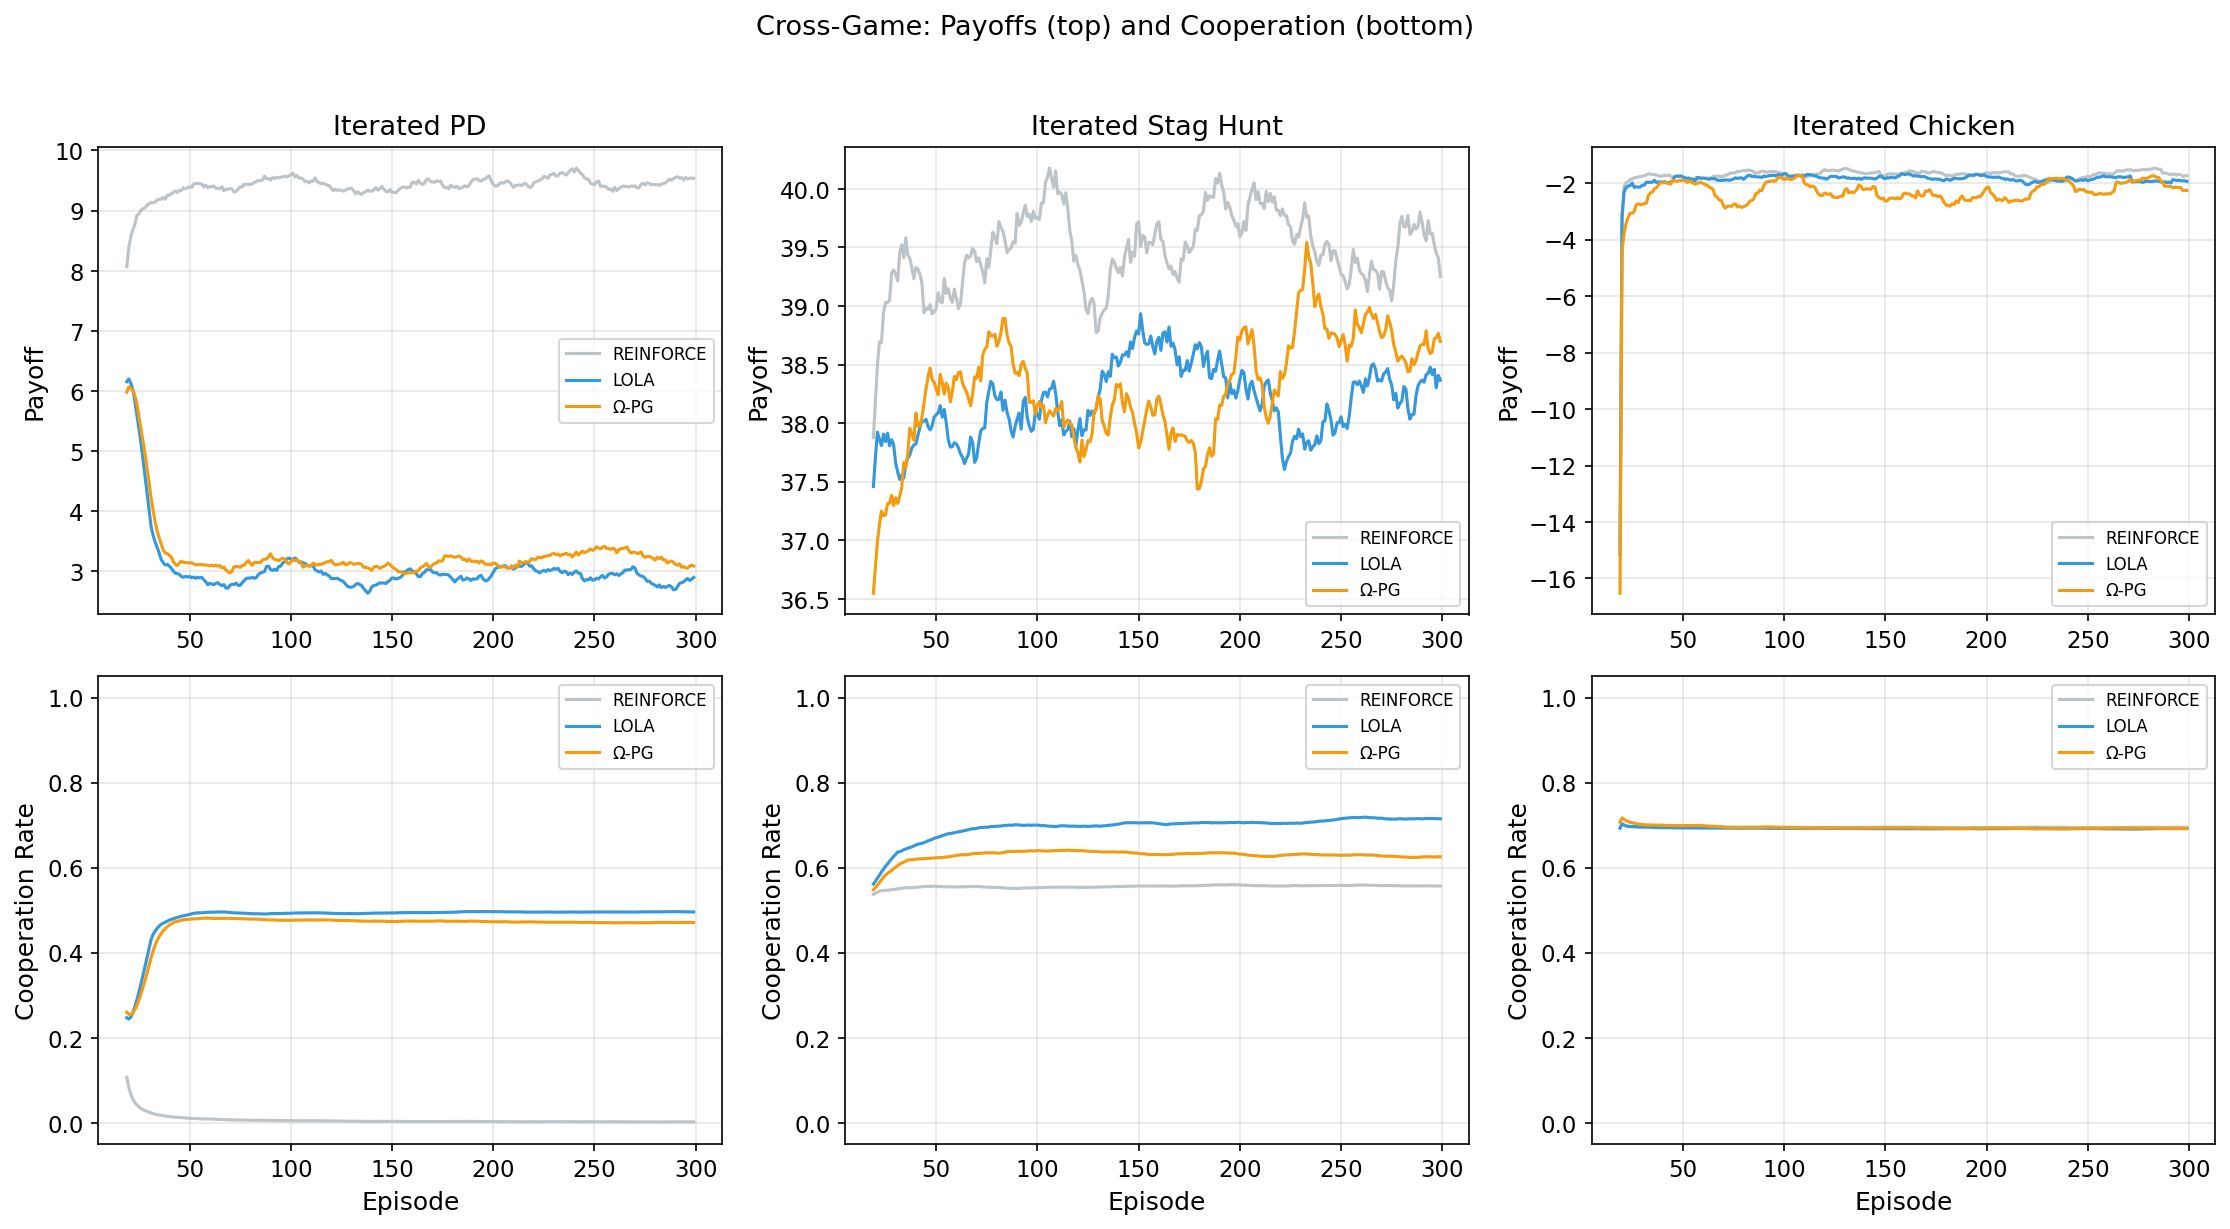
\includegraphics[width=\textwidth]{figures/iterated/cross_game.png}
\caption{Cross-game: payoffs (top) and cooperation rates (bottom) for IPD, Stag Hunt, Chicken.}
\label{fig:crossgame-app}
\end{figure}


\section{Discussion: The Cooperation Problem}

The strategy identification experiment reveals a fundamental limitation: \emph{per-episode policy gradient methods converge to the stage-game Nash equilibrium even in iterated games where better outcomes exist.} In the IPD, this means mutual defection.

This is not a failure of the $\Omega$-gradient but a \emph{theoretical result}: the SOS condition (Definition~\ref{def:sos}) guarantees convergence to NE, and defection \emph{is} the unique NE of the stage game. FP-NE correctly identifies this equilibrium. The problem is that the desirable cooperative outcomes (TFT, Pavlov) are not Nash equilibria of the stage game --- they are equilibria of the \emph{repeated} game under different solution concepts (subgame perfection with sufficiently high discount factor).

Three paths forward:
\begin{enumerate}
    \item \textbf{Meta-learning (Phase $-1$)}: optimise over the \emph{trajectory} of joint policy updates, as in Meta-MAPG~\cite{kim2021policygradientalgorithmlearning}. This adds a meta-value function over the $\Omega$-gradient's own dynamics.
    \item \textbf{FP-NE on the repeated game}: search for fixed points of the \emph{iterated} best-response map (5-state tabular policies), where TFT-like strategies are genuine NE.
    \item \textbf{Homotopy methods}: track the QRE correspondence as $\tau \to 0$, watching for bifurcation points where cooperative and defective equilibria separate.
\end{enumerate}
